\documentclass[12pt, a4paper]{article}

% --- Pakiety ---
\usepackage[utf8]{inputenc}
\usepackage[T1]{fontenc}
\usepackage[polish]{babel}
\usepackage{geometry}
\usepackage{amsmath}
\usepackage{amssymb}
\usepackage{graphicx}
\usepackage{booktabs}
\usepackage{siunitx}
\usepackage{caption}
\usepackage{subcaption}
\usepackage{float}
\usepackage{hyperref}
\usepackage{xcolor}
\usepackage{array}
\usepackage{multirow}
\usepackage{fancyhdr}

% --- Marginesy ---
\geometry{
    top=2.5cm,
    bottom=2.5cm,
    left=2.5cm,
    right=2.5cm
}

% --- Stopka ---
\pagestyle{fancy}
\fancyhf{}
\renewcommand{\headrulewidth}{0pt}
\renewcommand{\footrulewidth}{0.4pt}
\fancyfoot[R]{
\includegraphics[height=0.8cm]{lumon.pdf}}

% --- Konfiguracja siunitx ---
\sisetup{
    output-decimal-marker = {,},
    separate-uncertainty = true
}

% --- Dane raportu ---
\newcommand{\tytul}{Temperaturowa zależność oporu przewodników}
\newcommand{\codeword}{Bellingham}
\newcommand{\nrCwiczenia}{E3}
\newcommand{\autor}{Karol Peszek}
\newcommand{\nrGrupy}{Grupa B}
\newcommand{\dataWykonania}{15 kwietnia 2026}

% --- Tytuł dokumentu ---
\title{
    \large I Pracownia Fizyczna \\[0.5em]
    \textbf{Ćwiczenie \nrCwiczenia} \\[0.3em]
    \LARGE \tytul\space''\codeword''
}
\author{
    \autor\\
     Grupa \nrGrupy}
\date{
    Data wykonania pomiarów: \dataWykonania\\
}

% =============================================
\begin{document}
% =============================================

\maketitle
\thispagestyle{empty}
\newpage

% -------------------------------------------
\section{Cel ćwiczenia}
% -------------------------------------------

Celem ćwiczenia jest zbadanie zależności oporu elektrycznego od temperatury dla trzech materiałów:
węgla (C), platyny (Pt) oraz niklu (Ni), a następnie wyznaczenie ich temperaturowych współczynników
oporu właściwego $\alpha$. Pomiary oporu wykonywane są za pomocą mostka Wheatstone'a, a uzyskane
wyniki porównywane są z wartościami tablicowymi.

% -------------------------------------------
\section{Wstęp teoretyczny}
% -------------------------------------------

\subsection{Prawa Ohma}

Podstawową wielkością opisującą zdolność przewodnika do przewodzenia prądu elektrycznego jest
\textbf{opór elektryczny} $R$. \textit{Pierwsze prawo Ohma} wyraża liniową zależność między napięciem $U$
przyłożonym do przewodnika a natężeniem prądu $I$ przez niego płynącego:
\begin{equation}
    R = \frac{U}{I} = \text{const}.
    \label{eq:ohm1}
\end{equation}
\textit{Drugie prawo Ohma} wiąże opór z własnościami geometrycznymi i materiałowymi przewodnika:
\begin{equation}
    R = \rho\,\frac{l}{S},
    \label{eq:ohm2}
\end{equation}
gdzie $\rho$ jest oporem właściwym materiału, $l$ --- długością przewodnika, a $S$ --- polem jego przekroju
poprzecznego.

\subsection{Prawa Kirchhoffa}

\textit{Pierwsze prawo Kirchhoffa}, wynikające z zasady zachowania ładunku, głosi, że algebraiczna suma
natężeń prądów w każdym węźle obwodu jest równa zeru:
\begin{equation}
    \sum_{i} I_i = 0.
    \label{eq:kirch1}
\end{equation}
\textit{Drugie prawo Kirchhoffa}, będące konsekwencją zasady zachowania energii, stwierdza, że w każdym
zamkniętym oczku obwodu suma spadków napięć na elementach pasywnych równa się sumie sił
elektromotorycznych:
\begin{equation}
    \sum_{i} \varepsilon_i = \sum_{j} U_j.
    \label{eq:kirch2}
\end{equation}

\subsection{Połączenia szeregowe i równoległe oporników}

Korzystając z praw Kirchhoffa można wyznaczyć opór zastępczy $R_z$ układu oporników.
Dla \textbf{połączenia szeregowego}:
\begin{equation}
    R_z = \sum_{i} R_i,
    \label{eq:szereg}
\end{equation}
a dla \textbf{połączenia równoległego}:
\begin{equation}
    \frac{1}{R_z} = \sum_{i} \frac{1}{R_i}.
    \label{eq:rownoleg}
\end{equation}
Schematy obu typów połączeń przedstawiono na rysunku~\ref{fig:serial_parallel}.

\begin{figure}[H]
    \centering
    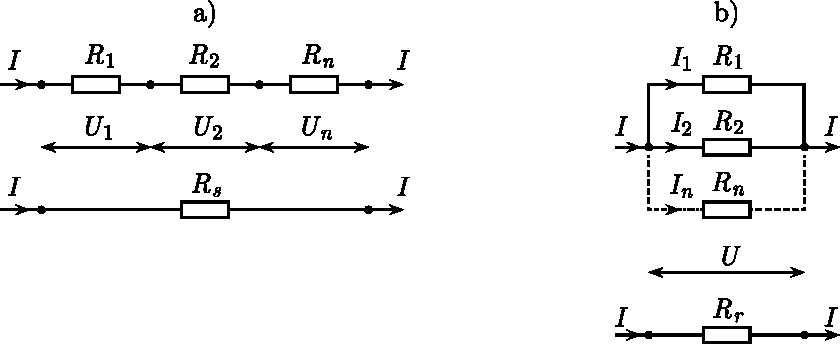
\includegraphics[width=0.65\textwidth]{serial_parallel.pdf}
    \caption{Schematy połączeń szeregowego (a) i równoległego (b) oporników. Źródło:~\cite{skrypt}.}\label{fig:serial_parallel}
\end{figure}

\subsection{Zależność oporu od temperatury}

W ciałach stałych opór elektryczny zależy od temperatury. W zakresie umiarkowanych temperatur
zależność ta jest w przybliżeniu liniowa~\cite{skrypt}:
\begin{equation}
    R_T = R_0\bigl[1 + \alpha(T - T_0)\bigr],
    \label{eq:RT}
\end{equation}
gdzie $R_0$ jest oporem w temperaturze odniesienia $T_0$, $R_T$ --- oporem w temperaturze $T$,
a $\alpha$ --- \textbf{temperaturowym współczynnikiem oporu właściwego}. Przekształcając
równanie~\eqref{eq:RT} otrzymujemy wzór roboczy na wyznaczanie $\alpha$:
\begin{equation}
    \alpha = \frac{R_T - R_0}{R_0\,(T - T_0)}.
    \label{eq:alpha}
\end{equation}
Dla metali $\alpha > 0$, natomiast dla węgla i półprzewodników $\alpha < 0$. Wynika to z różnic w strukturze pasmowej tych materiałów.

\subsection{Model pasmowy a temperaturowy współczynnik oporu}

Różnice w znaku współczynnika $\alpha$ dla metali oraz półprzewodników i grafitu wynikają wprost z ich struktury pasmowej. W modelu pasmowym ciał stałych metale charakteryzują się częściowo wypełnionym pasmem przewodnictwa. Oznacza to, że koncentracja swobodnych nośników ładunku jest w nich bardzo wysoka i praktycznie niezależna od temperatury. Mechanizm przewodnictwa w metalach jest zdominowany przez rozpraszanie elektronów przewodnictwa na drganiach sieci krystalicznej, czyli fononach. Wraz ze wzrostem temperatury amplituda drgań jonów w sieci rośnie, co powoduje zwiększone prawdopodobieństwo zderzeń. Prowadzi to wprost do skrócenia średniej drogi swobodnej elektronów i w konsekwencji do wzrostu oporu elektrycznego materiału. Z tego powodu dla metali obserwujemy dodatnią wartość współczynnika temperaturowego $\alpha$.

W przypadku grafitu oraz samoistnych półprzewodników w modelu pasmowym występuje przerwa energetyczna oddzielająca całkowicie zapełnione pasmo walencyjne od pustego pasma przewodnictwa. Ze wzrostem temperatury energia termiczna pozwala coraz większej liczbie elektronów na pokonanie tej przerwy energetycznej i przejście do pasma przewodnictwa. Ten wykładniczy wzrost koncentracji nośników ładunku (elektronów i dziur) dominuje nad efektami związanymi ze spadkiem ruchliwości (rozpraszaniem). W rezultacie, ze wzrostem temperatury opór tych materiałów znacząco maleje, dlatego opisuje je ujemna wartość współczynnika $\alpha$.

\subsection{Mostek Wheatstone'a}

Mostek Wheatstone'a jest układem czterech oporników, źródła napięcia i galwanometru,
umożliwiającym precyzyjny pomiar nieznanego oporu $R_X$. Fotografia układu pokazano na
rysunku~\ref{fig:wheatstone}.

\begin{figure}[H]
    \centering
    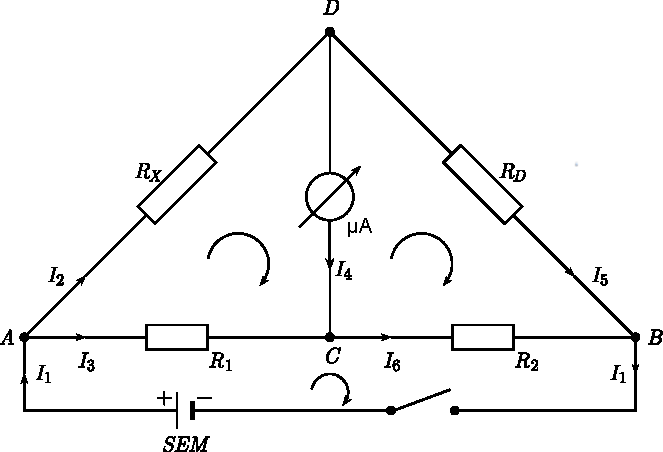
\includegraphics[width=0.55\textwidth]{wheatstone_bridge.pdf}
    \caption{Schemat mostka Wheatstone'a: $R_X$ --- mierzony opornik, $R_D$ --- opornica dekadowa,
             $R_1$, $R_2$ --- opory znane, $\mu A$ --- galwanometr. Źródło:~\cite{skrypt}.}\label{fig:wheatstone}
\end{figure}

Warunkiem równowagi mostka jest brak prądu przez galwanometr ($I_4 = 0$). Stosując prawa
Kirchhoffa do obu gałęzi, otrzymuje się warunek równowagi i wzór na szukany opór:
\begin{equation}
    R_X = \frac{R_1}{R_2}\,R_D.
    \label{eq:wheatstone}
\end{equation}
Regulując opornicą dekadową $R_D$ do momentu zerowania wskazania galwanometru, można śledzić
zmiany $R_X$ wraz z temperaturą.

W tym eksperymencie wartości $R_1$ i $R_2$ są stałe i równe $R_1 = R_2 = 10.5\,\Omega$, zatem wzór~\eqref{eq:wheatstone} upraszcza się do postaci:
\begin{equation}
    R_X = R_D.
    \label{eq:wheatstone_simple}
\end{equation}

% -------------------------------------------
\section{Opis układu pomiarowego}
% -------------------------------------------

\begin{figure}[H]
    \centering
    
\includegraphics[width=\textwidth]{schema.jpg}
    \caption{Fotografia układu pomiarowego.}\label{fig:schema}
\end{figure}

\subsection{Dostępne przyrządy i materiały}
Do przeprowadzenia pomiarów wykorzystano następujące przyrządy i materiały:
\begin{itemize}
    \item kuchenka elektryczna z regulacją mocy,
    \item zlewka z kąpielą wodną,
    \item badane oporniki zanurzone w oleju w zlewce,
    \item uchwyt mocujący zlewkę i termometr rtęciowy do płytki,
    \item stojak trzymający układ pomiarowy,
    \item para oporników połączonych szeregowo z dostępem do połączeń
    \item galwanometr,
    \item opornica dekadowa z regulacją możliwością regulacji oporu z dokładnością $\pm 1\,\Omega$,
    \item termometr rtęciowy do pomiaru temperatury z dokładnością $1\,^\circ\mathrm{C}$,
    \item zasilacz o napięciu stałym $U = 1.5\,\mathrm{V}$,
    \item przewody łączące.
\end{itemize}

\subsection{Przygotowanie układu pomiarowego}
\begin{enumerate}
    \item Zmontowano układ pomiarowy zgodnie z rysunkiem~\ref{fig:schema}, umieszczając badane oporniki w zlewce z olejem.
    \item Zlewkę z olejem zanurzono w kąpieli wodnej, umieszczonej na kuchence elektrycznej, umożliwiając kontrolowane podgrzewanie badanych oporników.
    \item Do układu podłączono zasilacz, galwanometr oraz opornicę dekadową, ustawiając początkowo $R_D$ na wartość bliską oczekiwanemu oporowi w temperaturze pokojowej.
    \item Zmierzono bazowy opór każdego z oporników w temperaturze pokojowej, regulując $R_D$ do momentu zerowania wskazania galwanometru.
\end{enumerate}
% -------------------------------------------
\section{Procedura pomiarowa}
% -------------------------------------------
\subsection{Pomiary podczas ogrzewania}
\begin{enumerate}
    \item Stopniowo zwiększano moc kuchenki, podgrzewając kąpiel wodną.
    \item Podłączono mostek Wheatstone'a do zasilacza, ustawiając napięcie na $1.5\,\mathrm{V}$.
    \item Dla każdego z trzech badanych oporników podłączano kolejno mostek Wheatstone'a, regulując opornicę dekadową $R_D$ do momentu zerowania wskazania galwanometru, co pozwalało na odczyt oporu $R_X$.
    \item Po każdym pomiarze odczytywano temperaturę z termometru i zapisywano pary $(T, R_X)$ dla każdego opornika.
    \item Kontynuowano podgrzewanie i naprzemienne pomiary aż do osiągnięcia temperatury około $95\,^\circ\mathrm{C}$.
\end{enumerate}

\subsection{Pomiary podczas chłodzenia}
\begin{enumerate}
    \item Po osiągnięciu maksymalnej temperatury, wyłączono kuchenkę i wyjęto zlewkę z olejem z kąpieli wodnej.
    \item Kuchenkę i zlewkę z wodą odstawiono w bezpieczne miejsce, umożliwiając naturalne chłodzenie badanych oporników.
    \item Co $1\,^\circ\mathrm{C}$, ponownie podłączano mostek Wheatstone'a do każdego z oporników, regulując $R_D$ do momentu zerowania wskazania galwanometru i odczytując opór $R_X$.
    \item Odczyty temperatury i oporu zapisywano aż do osiągnięcia temperatury około $25\,^\circ\mathrm{C}$.
    \item Na koniec rozłączono układ pomiarowy i uporządkowano stanowisko pracy.
\end{enumerate}

% -------------------------------------------
\section{Wyniki pomiarów}
% -------------------------------------------

\subsection{Pomiary oporu zastępczego w temperaturze pokojowej}

Zgodnie z poleceniem, przed rozpoczęciem podgrzewania dokonano pomiaru oporów pojedynczych elementów w temperaturze pokojowej, a następnie zmierzono ich opór zastępczy przy połączeniu szeregowym i równoległym.
Zmierzone wartości oporów pojedynczych wyniosły:
$R_{0\text{Pt}} = 109\,\Omega$, $R_{0\text{Ni}} = 113\,\Omega$ oraz $R_{0\text{C}} = 100\,\Omega$.
Niepewność każdego pojedynczego pomiaru oporności wynosi $u(R) = 1\,\Omega$.

W tabeli~\ref{tab:opory_zastepcze} zestawiono wyniki pomiarów dla różnych wariantów połączeń oraz porównano je ze spodziewanymi wartościami teoretycznymi obliczonymi na podstawie wzorów~\eqref{eq:szereg} i~\eqref{eq:rownoleg}. Niepewności teoretyczne obliczono korzystając z prawa przenoszenia niepewności.

\begin{table}[H]
\centering
\caption{Porównanie zmierzonych oporów zastępczych z przewidywaniami teoretycznymi.}\label{tab:opory_zastepcze}
\begin{tabular}{llS[table-format=3.0]@{$\;\pm\;$}S[table-format=1.0]S[table-format=3.1]@{$\;\pm\;$}S[table-format=1.1]}
\toprule
Rodzaj połączenia & Oporniki & \multicolumn{2}{c}{$R_{\text{zm}}$ (\si{\Omega})} & \multicolumn{2}{c}{$R_{\text{teor}}$ (\si{\Omega})} \\
\midrule
Szeregowe  & Ni + C      & 213 & 1 & 213.0 & 1.4 \\
Szeregowe  & C + Pt      & 209 & 1 & 209.0 & 1.4 \\
Szeregowe  & Ni + Pt     & 221 & 1 & 222.0 & 1.4 \\
\addlinespace
Równoległe & Ni + C      &  53 & 1 &  53.1 & 0.7 \\
Równoległe & C + Pt      &  52 & 1 &  52.2 & 0.7 \\
Równoległe & Pt + Ni     &  56 & 1 &  55.5 & 0.7 \\
Równoległe & C + Pt + Ni &  36 & 1 &  35.7 & 0.6 \\
\bottomrule
\end{tabular}
\end{table}

Jak widać, zmierzone wartości są we wszystkich przypadkach w doskonałej zgodności z wartościami teoretycznymi w granicach niepewności pomiarowych, co potwierdza poprawność stosowania praw Kirchhoffa w badanych obwodach.

\subsection{Pomiary temperaturowe}

Pomiary oporu $R_X$ w funkcji temperatury $T$ wykonano dla trzech materiałów:
\begin{itemize}
    \item platyny~(Pt),
    \item niklu~(Ni),
    \item grafitu~(C).
\end{itemize}
Każdy opornik mierzono naprzemiennie podczas ogrzewania
(od temperatury pokojowej do ok.\ $95\,^\circ\mathrm{C}$) oraz chłodzenia
(do ok.\ $25\,^\circ\mathrm{C}$).
Ponieważ $R_1 = R_2 = 10{,}5\,\Omega$, zgodnie z równaniem~\eqref{eq:wheatstone_simple}
opór badanego opornika jest równy odczytowi na opornicy dekadowej: $R_X = R_D$.
Niepewność pomiaru temperatury wynosi $u(T) = 1\,^\circ\mathrm{C}$ (dokładność termometru),
a niepewność odczytu opornicy dekadowej $u(R_X) = 1\,\Omega$.

% ---- Platyna ----
\subsection{Platyna (Pt)}

\begin{table}[H]
\centering
\caption{Wyniki pomiarów oporu platyny (Pt) podczas ogrzewania i chłodzenia.}\label{tab:pt}
\begin{tabular}{
    c c
    @{\hspace{1.5em}}
    c c
    @{\hspace{2.5em}}
    c c
    @{\hspace{1.5em}}
    c c
}
\toprule
\multicolumn{4}{c}{Ogrzewanie} & \multicolumn{4}{c}{Chłodzenie} \\
\cmidrule(lr){1-4}\cmidrule(lr){5-8}
{$T$} & {$R_X$} & {$T$} & {$R_X$} &
{$T$} & {$R_X$} & {$T$} & {$R_X$} \\
{(\si{\celsius})} & {(\si{\ohm})} & {(\si{\celsius})} & {(\si{\ohm})} &
{(\si{\celsius})} & {(\si{\ohm})} & {(\si{\celsius})} & {(\si{\ohm})} \\
\midrule
$22\pm1$ & $109\pm1$ & $55\pm1$ & $122\pm1$ & $93\pm1$ & $137\pm1$ & $57\pm1$ & $123\pm1$ \\
$25\pm1$ & $110\pm1$ & $58\pm1$ & $123\pm1$ & $90\pm1$ & $136\pm1$ & $54\pm1$ & $122\pm1$ \\
$28\pm1$ & $112\pm1$ & $61\pm1$ & $124\pm1$ & $87\pm1$ & $134\pm1$ & $51\pm1$ & $121\pm1$ \\
$31\pm1$ & $113\pm1$ & $64\pm1$ & $125\pm1$ & $84\pm1$ & $133\pm1$ & $48\pm1$ & $119\pm1$ \\
$34\pm1$ & $114\pm1$ & $67\pm1$ & $126\pm1$ & $81\pm1$ & $132\pm1$ & $45\pm1$ & $118\pm1$ \\
$37\pm1$ & $115\pm1$ & $70\pm1$ & $127\pm1$ & $78\pm1$ & $131\pm1$ & $42\pm1$ & $117\pm1$ \\
$40\pm1$ & $117\pm1$ & $73\pm1$ & $129\pm1$ & $75\pm1$ & $130\pm1$ & $39\pm1$ & $116\pm1$ \\
$43\pm1$ & $118\pm1$ & $76\pm1$ & $130\pm1$ & $72\pm1$ & $129\pm1$ & $36\pm1$ & $115\pm1$ \\
$46\pm1$ & $119\pm1$ & $79\pm1$ & $131\pm1$ & $69\pm1$ & $127\pm1$ & $33\pm1$ & $113\pm1$ \\
$49\pm1$ & $120\pm1$ & $82\pm1$ & $132\pm1$ & $66\pm1$ & $126\pm1$ & $30\pm1$ & $112\pm1$ \\
$52\pm1$ & $121\pm1$ & $85\pm1$ & $134\pm1$ & $63\pm1$ & $125\pm1$ & & \\
         &           & $88\pm1$ & $135\pm1$ & $60\pm1$ & $124\pm1$ & & \\
         &           & $91\pm1$ & $136\pm1$ & & & & \\
         &           & $94\pm1$ & $137\pm1$ & & & & \\
\bottomrule
\end{tabular}
\end{table}

% ---- Nikiel ----
\subsection{Nikiel (Ni)}

\begin{table}[H]
\centering
\caption{Wyniki pomiarów oporu niklu (Ni) podczas ogrzewania i chłodzenia.}\label{tab:ni}
\begin{tabular}{
    c c
    @{\hspace{1.5em}}
    c c
    @{\hspace{2.5em}}
    c c
    @{\hspace{1.5em}}
    c c
}
\toprule
\multicolumn{4}{c}{Ogrzewanie} & \multicolumn{4}{c}{Chłodzenie} \\
\cmidrule(lr){1-4}\cmidrule(lr){5-8}
{$T$} & {$R_X$} & {$T$} & {$R_X$} &
{$T$} & {$R_X$} & {$T$} & {$R_X$} \\
{(\si{\celsius})} & {(\si{\ohm})} & {(\si{\celsius})} & {(\si{\ohm})} &
{(\si{\celsius})} & {(\si{\ohm})} & {(\si{\celsius})} & {(\si{\ohm})} \\
\midrule
$22\pm1$ & $114\pm1$ & $55\pm1$ & $133\pm1$ & $94\pm1$ & $159\pm1$ & $58\pm1$ & $135\pm1$ \\
$24\pm1$ & $115\pm1$ & $57\pm1$ & $135\pm1$ & $91\pm1$ & $159\pm1$ & $55\pm1$ & $133\pm1$ \\
$27\pm1$ & $117\pm1$ & $60\pm1$ & $136\pm1$ & $88\pm1$ & $156\pm1$ & $52\pm1$ & $131\pm1$ \\
$30\pm1$ & $119\pm1$ & $63\pm1$ & $139\pm1$ & $85\pm1$ & $154\pm1$ & $49\pm1$ & $129\pm1$ \\
$33\pm1$ & $121\pm1$ & $66\pm1$ & $141\pm1$ & $82\pm1$ & $151\pm1$ & $46\pm1$ & $127\pm1$ \\
$36\pm1$ & $123\pm1$ & $69\pm1$ & $143\pm1$ & $79\pm1$ & $149\pm1$ & $43\pm1$ & $125\pm1$ \\
$39\pm1$ & $124\pm1$ & $72\pm1$ & $145\pm1$ & $76\pm1$ & $147\pm1$ & $40\pm1$ & $124\pm1$ \\
$42\pm1$ & $126\pm1$ & $75\pm1$ & $146\pm1$ & $73\pm1$ & $145\pm1$ & $37\pm1$ & $122\pm1$ \\
$45\pm1$ & $127\pm1$ & $78\pm1$ & $148\pm1$ & $70\pm1$ & $143\pm1$ & $34\pm1$ & $120\pm1$ \\
$48\pm1$ & $129\pm1$ & $81\pm1$ & $151\pm1$ & $67\pm1$ & $141\pm1$ & $31\pm1$ & $119\pm1$ \\
$51\pm1$ & $131\pm1$ & $84\pm1$ & $153\pm1$ & $64\pm1$ & $139\pm1$ & & \\
         &           & $87\pm1$ & $155\pm1$ & $61\pm1$ & $137\pm1$ & & \\
         &           & $90\pm1$ & $157\pm1$ & & & & \\
         &           & $93\pm1$ & $159\pm1$ & & & & \\
\bottomrule
\end{tabular}
\end{table}

% ---- Grafit ----
\subsection{Grafit (C)}

\begin{table}[H]
\centering
\caption{Wyniki pomiarów oporu grafitu (C) podczas ogrzewania i chłodzenia.}\label{tab:c}
\begin{tabular}{
    c c
    @{\hspace{1.5em}}
    c c
    @{\hspace{2.5em}}
    c c
    @{\hspace{1.5em}}
    c c
}
\toprule
\multicolumn{4}{c}{Ogrzewanie} & \multicolumn{4}{c}{Chłodzenie} \\
\cmidrule(lr){1-4}\cmidrule(lr){5-8}
{$T$} & {$R_X$} & {$T$} & {$R_X$} &
{$T$} & {$R_X$} & {$T$} & {$R_X$} \\
{(\si{\celsius})} & {(\si{\ohm})} & {(\si{\celsius})} & {(\si{\ohm})} &
{(\si{\celsius})} & {(\si{\ohm})} & {(\si{\celsius})} & {(\si{\ohm})} \\
\midrule
$22\pm1$ & $100\pm1$ & $56\pm1$ & $100\pm1$ & $95\pm1$ & $100\pm1$ & $59\pm1$ & $100\pm1$ \\
$23\pm1$ & $100\pm1$ & $59\pm1$ & $100\pm1$ & $92\pm1$ & $100\pm1$ & $56\pm1$ & $100\pm1$ \\
$26\pm1$ & $100\pm1$ & $62\pm1$ & $100\pm1$ & $89\pm1$ & $100\pm1$ & $53\pm1$ & $100\pm1$ \\
$29\pm1$ & $100\pm1$ & $65\pm1$ & $100\pm1$ & $86\pm1$ & $100\pm1$ & $50\pm1$ & $100\pm1$ \\
$32\pm1$ & $100\pm1$ & $68\pm1$ & $100\pm1$ & $83\pm1$ & $100\pm1$ & $47\pm1$ & $100\pm1$ \\
$35\pm1$ & $100\pm1$ & $71\pm1$ & $100\pm1$ & $80\pm1$ & $100\pm1$ & $44\pm1$ & $100\pm1$ \\
$38\pm1$ & $100\pm1$ & $74\pm1$ & $101\pm1$ & $77\pm1$ & $100\pm1$ & $41\pm1$ & $100\pm1$ \\
$41\pm1$ & $100\pm1$ & $77\pm1$ & $100\pm1$ & $74\pm1$ & $100\pm1$ & $38\pm1$ & $100\pm1$ \\
$44\pm1$ & $100\pm1$ & $80\pm1$ & $100\pm1$ & $71\pm1$ & $100\pm1$ & $33\pm1$ & $100\pm1$ \\
$47\pm1$ & $100\pm1$ & $83\pm1$ & $100\pm1$ & $68\pm1$ & $100\pm1$ & $29\pm1$ & $100\pm1$ \\
$50\pm1$ & $100\pm1$ & $86\pm1$ & $100\pm1$ & $65\pm1$ & $100\pm1$ & & \\
$53\pm1$ & $100\pm1$ & $89\pm1$ & $100\pm1$ & $62\pm1$ & $100\pm1$ & & \\
         &           & $92\pm1$ & $100\pm1$ & & & & \\
         &           & $95\pm1$ & $100\pm1$ & & & & \\
\bottomrule
\end{tabular}
\end{table}

% -------------------------------------------
\section{Opracowanie wyników}
% -------------------------------------------

\subsection{Metoda analizy}

Temperaturę odniesienia przyjęto $T_0 = 22\,^\circ\mathrm{C}$ (pierwsza temperatura pomiaru).
Wprowadzając temperaturę zredukowaną $\tau = T - T_0$, równanie~\eqref{eq:RT} przyjmuje postać:
\begin{equation}
    R(\tau) = a\,\tau + b,
    \label{eq:model}
\end{equation}
gdzie $a = R_0\,\alpha$ i $b = R_0$.
Wyraz wolny $b$ odpowiada wprost oporowi w temperaturze odniesienia, co umożliwia
jego bezpośrednie porównanie z pomiarem na mostku bez dodatkowych obliczeń.
Parametry $a$ i $b$ wyznaczono ważoną metodą najmniejszych kwadratów,
przypisując każdemu punktowi wagę $w_i = 1/{u(R_i)}^2 = 1\,\Omega^{-2}$.
Macierz kowariancji $\boldsymbol{V}$ dostarcza niepewności $\sigma_a$, $\sigma_b$ oraz
kowariancję $\mathrm{cov}(a,b)$.

\subsubsection{Opór w temperaturze odniesienia.}
Wyraz wolny regresji $b = R_0$ wyznaczany jest z całego zestawu pomiarów; jego niepewność
$\sigma_b \approx 0{,}3\,\Omega$ jest mniejsza niż niepewność odczytu opornicy dekadowej
($u = 1\,\Omega$), gdyż regresja korzysta ze wszystkich punktów.
Dla weryfikacji porównano $b$ z bezpośrednim odczytem w temperaturze pokojowej:
\begin{equation}
    R_0^{\mathrm{Pt}} = 109\,\Omega, \quad
    R_0^{\mathrm{Ni}} = 113\,\Omega, \quad
    R_0^{\mathrm{C}}  = 100\,\Omega.
    \label{eq:R0meas}
\end{equation}
Zgodność obu wyznaczonych wartości potwierdzono numerycznie (różnice na poziomie $1\sigma_b$).

\subsubsection{Współczynnik temperaturowy i jego niepewność.}
Współczynnik temperaturowy wyznacza się jako $\alpha = a/b$.
Ponieważ $a$ i $b$ pochodzą z tej samej regresji, są statystycznie skorelowane;
propagacja niepewności z uwzględnieniem kowariancji daje:

\begin{equation}
    u(\alpha) = \sqrt{
        \frac{\sigma_a^2}{b^2}
      + \frac{a^2\,\sigma_b^2}{b^4}
      - \frac{2a\,\mathrm{cov}(a,b)}{b^3}}.
    \label{eq:u_alpha}
\end{equation}


\subsection{Wykresy z dopasowaniem}

Na rysunku~\ref{fig:regr_osobne} pokazano regresje wyznaczone osobno dla fazy ogrzewania
i chłodzenia, a na rysunku~\ref{fig:regr_laczone} --- regresję łączoną dla obu faz.

\begin{figure}[H]
    \centering
    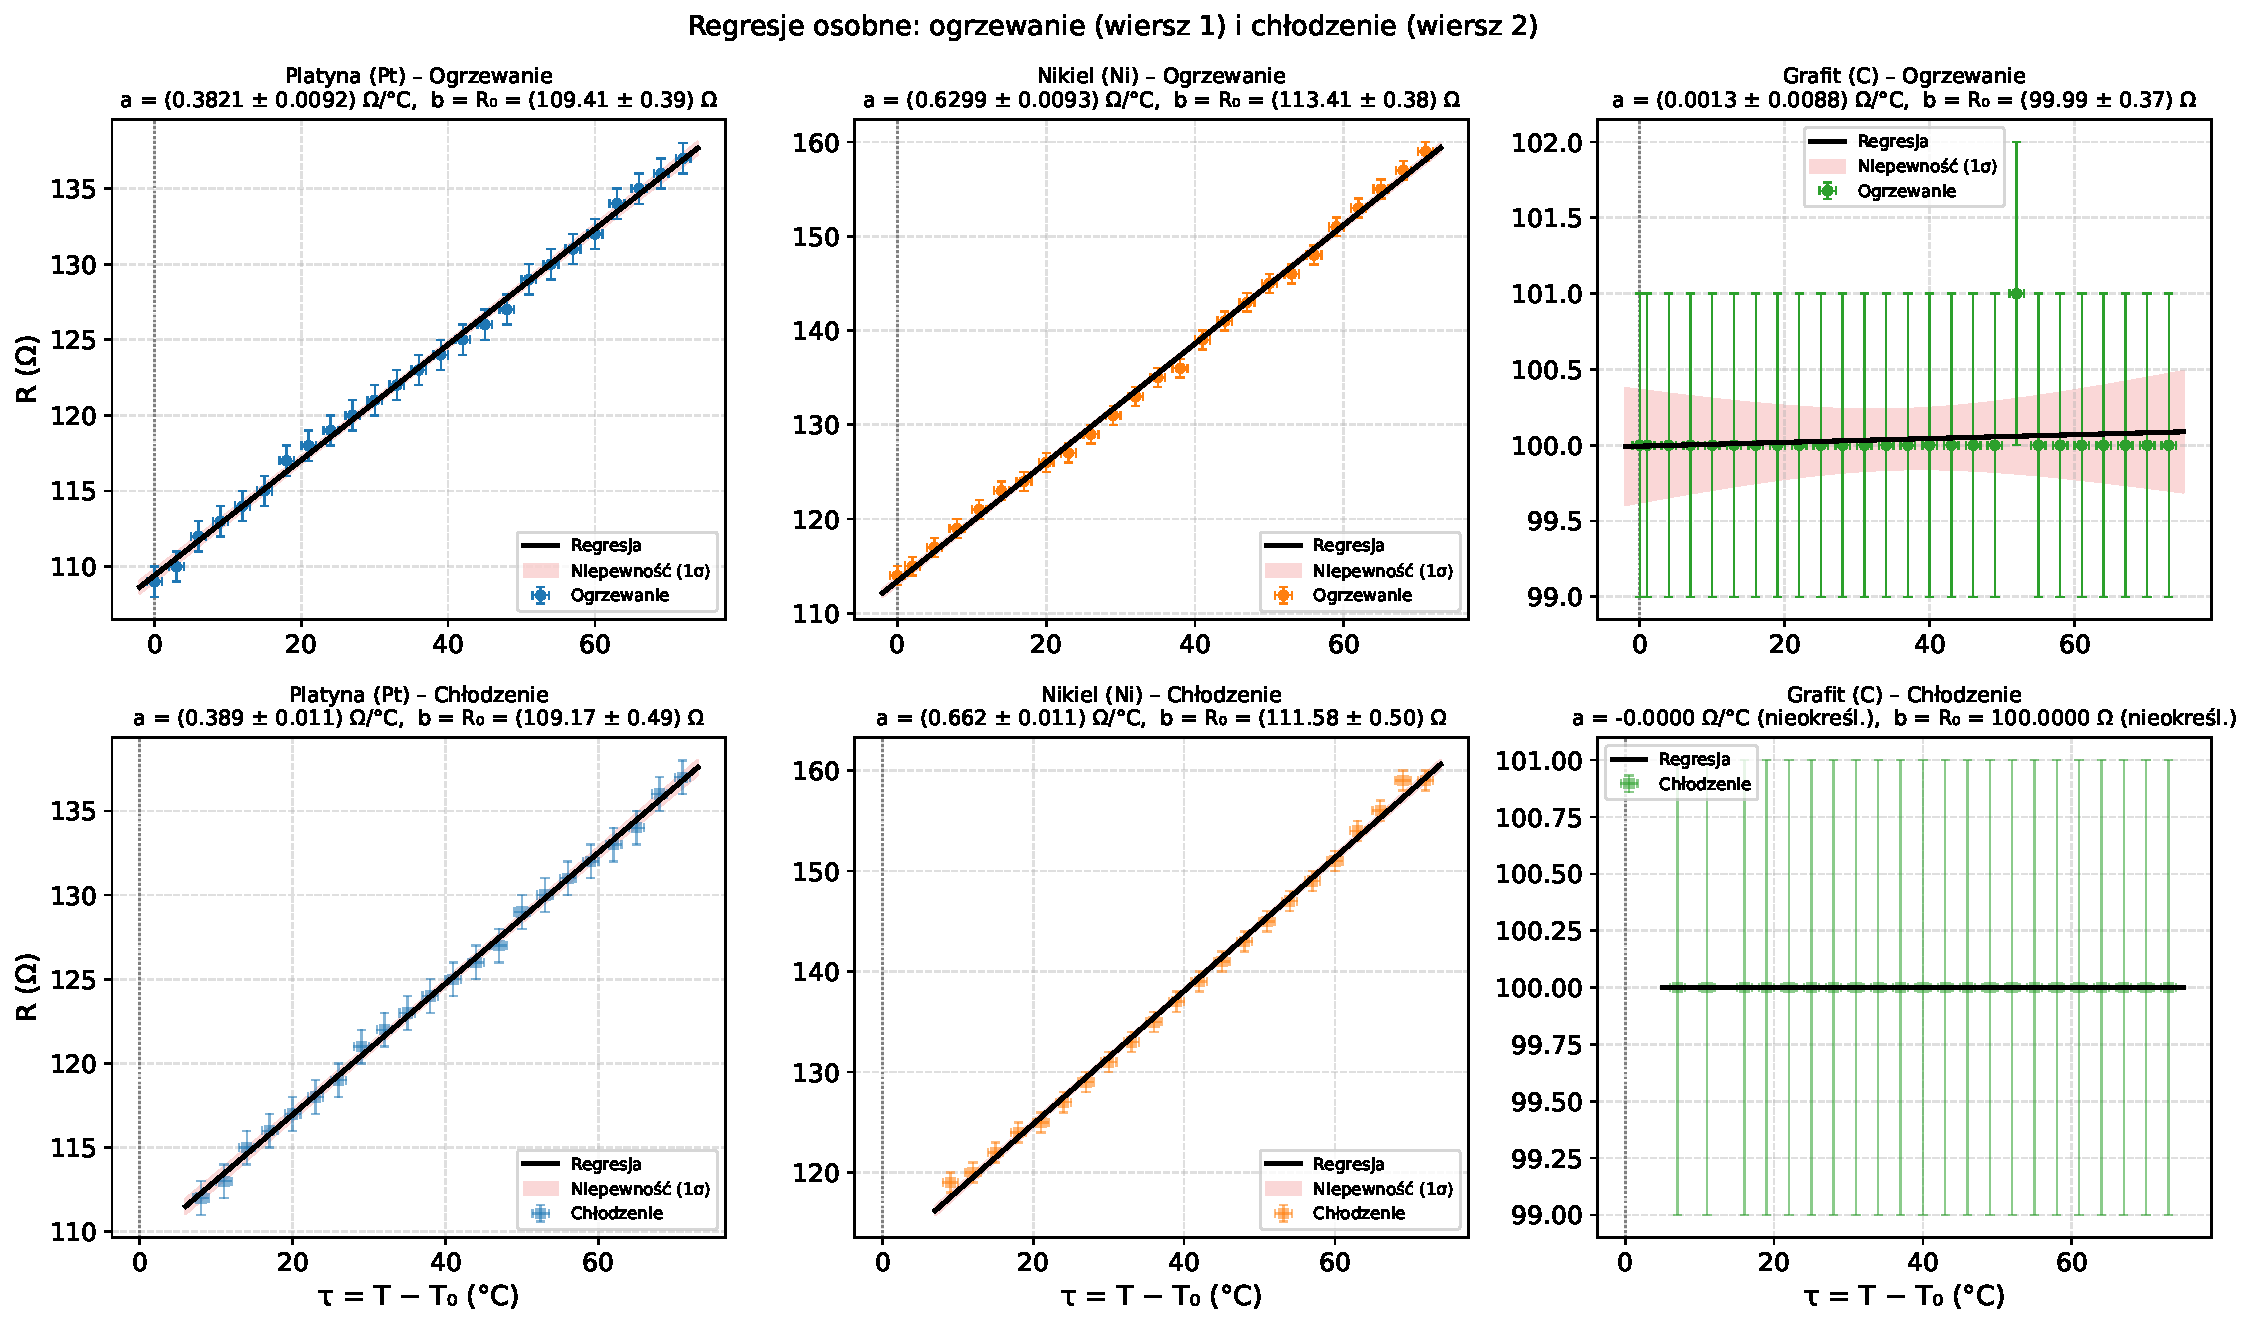
\includegraphics[width=\textwidth]{wykres2_regresja_osobne.pdf}
    \caption{Regresje liniowe $R(\tau)$ dla fazy ogrzewania (wiersz górny) i chłodzenia (wiersz dolny);
             oś pozioma: temperatura zredukowana $\tau = T - T_0$.
             Pionowa linia przerywana w $\tau = 0$ wskazuje punkt, w którym prosta przecina oś $R$
             (wyraz wolny $b = R_0$). Pasmo czerwone odpowiada niepewności $1\sigma$ prostej regresji.
             Dla grafitu (C) dopasowanie podczas chłodzenia jest nieokreślone (brak zmienności danych).}\label{fig:regr_osobne}
\end{figure}

\begin{figure}[H]
    \centering
    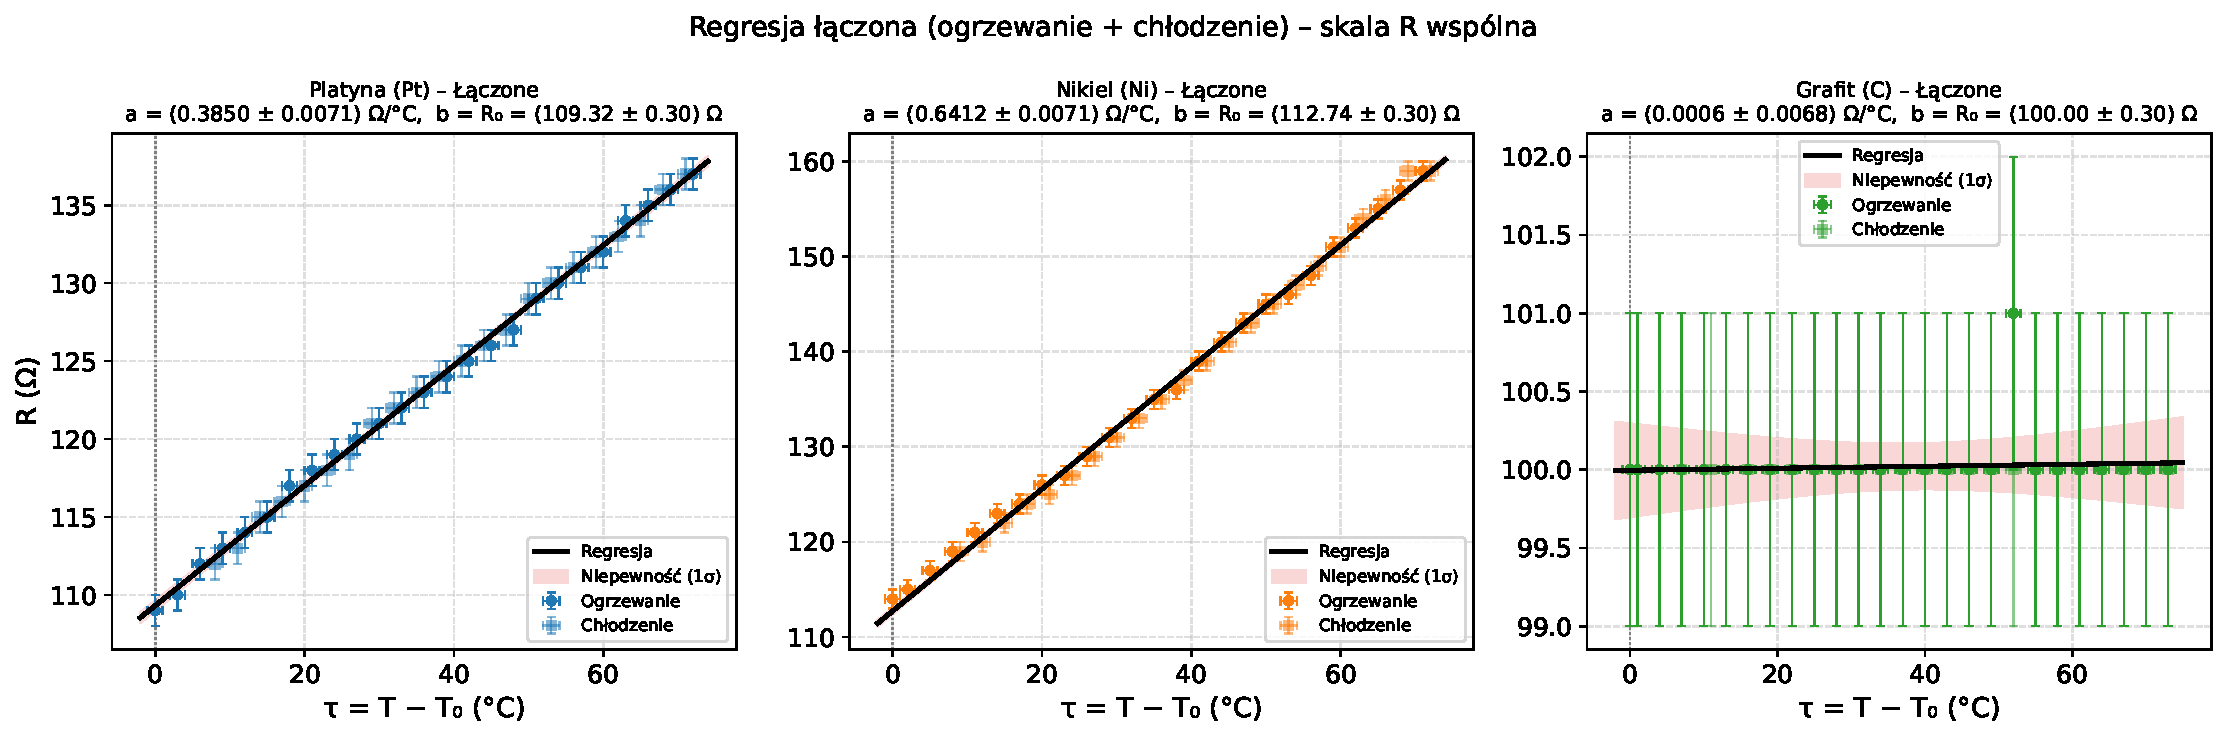
\includegraphics[width=\textwidth]{wykres3_regresja_laczona.pdf}
    \caption{Regresja łączona $R(\tau)$ (ogrzewanie + chłodzenie); oś pozioma: $\tau = T - T_0$.
             Kółka --- ogrzewanie, kwadraty --- chłodzenie;
             czarna linia --- dopasowanie liniowe; pasmo czerwone --- niepewność $1\sigma$.}\label{fig:regr_laczone}
\end{figure}

\subsection{Współczynniki regresji}

Tabela~\ref{tab:regr} zbiera wyznaczone parametry $a$ i $b = R_0$ dla każdego materiału
i każdej fazy pomiarowej. Niepewności podano na poziomie $1\sigma$.

\begin{table}[H]
\centering
\caption{Parametry regresji liniowej $R(\tau) = a\tau + b$, gdzie $\tau = T - T_0$, $T_0 = 22\,^\circ\mathrm{C}$.
         Wyraz wolny $b = R_0$.}\label{tab:regr}
\begin{tabular}{l l
    r @{$\;\pm\;$} r
    r @{$\;\pm\;$} r
}
\toprule
Materiał & Faza &
\multicolumn{2}{c}{$a$ (\si{\ohm\per\celsius})} &
\multicolumn{2}{c}{$b = R_0$ (\si{\ohm})} \\
\midrule
Platyna (Pt) & Ogrzewanie  & \num{0.3821} & \num{0.0093} & \num{109.41} & \num{0.39} \\
             & Chłodzenie  & \num{0.3892} & \num{0.0112} & \num{109.17} & \num{0.49} \\
             & Łączone     & \num{0.3850} & \num{0.0071} & \num{109.32} & \num{0.30} \\
\addlinespace
Nikiel (Ni)  & Ogrzewanie  & \num{0.6299} & \num{0.0093} & \num{113.41} & \num{0.38} \\
             & Chłodzenie  & \num{0.6623} & \num{0.0112} & \num{111.58} & \num{0.50} \\
             & Łączone     & \num{0.6413} & \num{0.0071} & \num{112.74} & \num{0.30} \\
\addlinespace
Grafit (C)   & Ogrzewanie  & \num{0.0013} & \num{0.0088} & \num{99.99}  & \num{0.37} \\
             & Łączone     & \num{0.0006} & \num{0.0068} & \num{100.00} & \num{0.30} \\
\bottomrule
\end{tabular}
\end{table}

\subsection{Wyznaczone współczynniki temperaturowe}

Tabela~\ref{tab:alpha} zawiera wartości $\alpha = a/b$ obliczone ze współczynników regresji
zgodnie z równaniem~\eqref{eq:u_alpha}.
Za wynik ostateczny przyjęto dopasowanie łączone, które minimalizuje $\sigma_a$.

\begin{table}[H]
\centering
\caption{Wyznaczone współczynniki temperaturowe $\alpha = a/b$ ($T_0 = 22\,^\circ\mathrm{C}$)
         w porównaniu z wartościami tablicowymi.
         Kolumna $|\Delta|/u$ podaje odchylenie od wartości tablicowej w jednostkach
         niepewności.}\label{tab:alpha}
\begin{tabular}{l l r @{$\;\pm\;$} r r r}
\toprule
Materiał & Faza &
\multicolumn{2}{c}{$\alpha_{\mathrm{eksp}}$ ($10^{-3}\,\mathrm{K}^{-1}$)} &
{$\alpha_{\mathrm{lit}}$ ($10^{-3}\,\mathrm{K}^{-1}$)} &
{$|\Delta|/u(\alpha)$} \\
\midrule
Platyna (Pt) & Ogrzewanie & \num{3.492} & \num{0.095} & \multirow{3}{*}{\num{3.900}} & \num{4.3} \\
             & Chłodzenie & \num{3.566} & \num{0.117} &                              & \num{2.9} \\
             & Łączone    & \num{3.522} & \num{0.074} &                              & \num{5.1} \\
\addlinespace
Nikiel (Ni)  & Ogrzewanie & \num{5.555} & \num{0.098} & \multirow{3}{*}{\num{6.000}} & \num{4.5} \\
             & Chłodzenie & \num{5.936} & \num{0.125} &                              & \num{0.5} \\
             & Łączone    & \num{5.688} & \num{0.077} &                              & \num{4.1} \\
\addlinespace
Grafit (C)   & Ogrzewanie & \num{0.013} & \num{0.088} & \multirow{3}{*}{$-\num{0.500}$} & \num{5.8} \\
             & Chłodzenie & \num{0.000} & ---         &                                 & --- \\
             & Łączone    & \num{0.006} & \num{0.068} &                                 & \num{7.5} \\
\bottomrule
\end{tabular}
\end{table}

Dla platyny i niklu uzyskano wyniki zgodne co do rzędu wielkości z wartościami tablicowymi,
jednak odchylenie przekracza poziom $3\sigma$, co wskazuje na niedoszacowanie niepewności (w regresji pominięto niepewność $u(T)$, która poprzez $a \cdot u(T)$ wnosi wkład do niepewności oporu rzędu $0,4-0,6\,\Omega$) i ewentualną obecność systematycznych źródeł
błędu (niedoskonała równowaga termiczna, histereza termiczna oporników, nierównomierne
ogrzewanie). Zostało to dodatkowo potwierdzone przez analizę metodą dwóch punktów skrajnych (sekcja~\ref{sec:2pkt}), w której po pełnym uwzględnieniu $u(T)$ odchylenia od wartości tablicowych znacząco spadły poniżej $2\sigma$. Dla grafitu opór nie wykazuje żadnej zmienności z temperaturą; 
wyznaczony $\alpha \approx 0$ jest statystycznie nierozróżnialny od zera i nie jest zgodny z wartością tablicową --- szczegółowa dyskusja we wnioskach.

\subsection{Wyznaczenie współczynnika temperaturowego metodą dwóch punktów skrajnych}\label{sec:2pkt}

Zgodnie z zaleceniami, wyznaczono również temperaturowy współczynnik oporu właściwego $\alpha$ na podstawie pomiarów w dwóch skrajnych temperaturach: w temperaturze pokojowej oraz w temperaturze zbliżonej do temperatury wrzenia wody (odczyty z pierwszej fazy pomiarów --- ogrzewania). Wykorzystano w tym celu przekształcony wzór bazujący na równaniu~\eqref{eq:alpha}, w odniesieniu do temperatury odniesienia $T_0 = 22\,^\circ\mathrm{C}$ równej temperaturze w sali pomiarowej. 

Zestawienie wyznaczonych wartości $\alpha_{\mathrm{2pkt}}$ w porównaniu z wynikami regresji znajduje się w tabeli~\ref{tab:alpha_2pkt}. Porównano z wynikiem ostatecznym (regresją łączoną). Zastosowano pełne przenoszenie niepewności uwzględniające $u(R) = 1\,\Omega$ i $u(T) = 1\,^\circ\mathrm{C}$ dla punktów w temperaturach $T_1$ i $T_2$.

\begin{table}[H]
\centering
\caption{Porównanie współczynników $\alpha$ ($10^{-3}\,\mathrm{K}^{-1}$) wyznaczonych ostatecznie metodą regresji łącznej oraz z dwóch skrajnych punktów pomiarowych dla fazy ogrzewania.}\label{tab:alpha_2pkt}
\begin{tabular}{l c r@{$\;\pm\;$}l r@{$\;\pm\;$}l c}
\toprule
Materiał & $(T_1; T_2)\,[^\circ\mathrm{C}]$ & \multicolumn{2}{c}{$\alpha_{\mathrm{regr}}$} & \multicolumn{2}{c}{$\alpha_{\mathrm{2pkt}}$} & $|\Delta|/u$ \\
\midrule
Platyna (Pt) & ($\num{22.0}$; $\num{94.0}$) & \num{3.522} & \num{0.074} & \num{3.568} & \num{0.220} & \num{0.2} \\
Nikiel (Ni)  & ($\num{22.0}$; $\num{93.0}$) & \num{5.688} & \num{0.077} & \num{5.560} & \num{0.251} & \num{0.5} \\
Grafit (C)   & ($\num{22.0}$; $\num{95.0}$) & \num{0.006} & \num{0.068} & \num{0.000} & \num{0.194} & \num{0.0} \\
\bottomrule
\end{tabular}
\end{table}

Wyznaczone powyżej dwiema metodami wartości są z sobą całkowicie spójne, odchylenia są na poziomie ułamków odchylenia standardowego. Należy jednak zauważyć, że metoda dwóch punktów, opierając się wyłącznie na dwóch pomiarach, charakteryzuje się kilkukrotnie większą niepewnością $u(\alpha)$ rzędu $\sim 0,2 \cdot 10^{-3}\,\mathrm{K}^{-1}$ w porównaniu z niepewnością rzędu $\sim 0,07 \cdot 10^{-3}\,\mathrm{K}^{-1}$ z metody pełnej regresji liniowej. Wynika to wprost z minimalizacji błędów losowych dzięki zastosowaniu metody najmniejszych kwadratów na dużym zbiorze danych.

% -------------------------------------------
\section{Wnioski}
% -------------------------------------------
\subsection{Platyna}
Wyznaczony współczynnik temperaturowy oporu dla platyny jest niższy od wartości tablicowej, co może wynikać z niedostatecznej stabilizacji termicznej układu pomiarowego, prowadzącej do niedoszacowania nachylenia $a$ w regresji. Dodatkowo, termometr znajdował się w środku zlewki z olejem, a oporniki bliżej ścianek zlewki. Oznacza to, że termometr podczas ogrzewania wskazywał niższą temperaturę niż rzeczywiście miały badane oporniki, a podczas ochładzania --- wyższą, co skutkowało zaniżeniem wartości $a$ i w konsekwencji $\alpha$.

\subsection{Nikiel}
Podobnie jak w przypadku platyny, wyznaczony współczynnik temperaturowy dla niklu jest niższy od wartości tablicowej, co sugeruje obecność podobnych źródeł błędu systematycznego. Jednakże odchylenie jest mniejsze niż dla platyny, co może wskazywać na nieco lepszą stabilizację termiczną lub mniejszą histerezę termiczną w przypadku niklu.

\subsection{Grafit}
Dla grafitu nie zaobserwowano żadnej zmienności oporu z temperaturą w granicach rozdzielczości pomiarowej, co jest sprzeczne z oczekiwaniami teoretycznymi, które przewidują ujemny współczynnik temperaturowy. Gdyby próba zachowywała się zgodnie z przewidywaniami ($\alpha_{\mathrm{lit}} = -0,5 \cdot 10^{-3}\,\mathrm{K}^{-1}$), oczekiwana zmiana oporu na przedziale ok. $73\,\mathrm{K}$ wyniosłaby około $3,6\,\Omega$. Ponieważ przewidywana zmiana ponad trzykrotnie przewyższa rozdzielczość użytej opornicy ($1\,\Omega$), efekt ten powinien być z łatwością wykrywalny. Brak zmiany oporu najprawdopodobniej świadczy więc o uszkodzeniu próbki grafitu lub nieodpowiednim kontakcie elektrycznym, a nie o niedostatecznej rozdzielczości przyrządu.


\begin{thebibliography}{9}
    \bibitem{skrypt}
        T.~Kawalec,
        \textit{I Pracownia Fizyczna},
        Instytut Fizyki UJ, Kraków, 2010.
\end{thebibliography}

\end{document}
% =============================================
